\section{Forundersøgelse}\label{ch:forundersoegelse}

\subsection{Medarbjeder-mål Tabel}
\begin{center}
\begin{longtable}{ |p{90pt}|p{90pt}|p{90pt}|p{90pt}| }
    \hline
    Medarbjeder & Opgave & Mål & Trin \\
    \hline\hline
    Ismand
    & Modtager ny ordre & Ordren er registreret som værende solgt. &
    - modtag ordre fra kunde \\
    &&&
    - Ordren med tilhørende adresse  registreres \\
    &&&
    - Adressen på ordren printes ud og lægges i den rigtige kasse til næste dag \\
    &&&
    - Den udprintede ordre tages med i bilen \\
    &&&
    - Ordren leveres til kunden på turen \\
    &&&
    - Kunden underskriver ordren \\
    &&&
    - Den underskrevene ordre afleveres til chefen \\
    \hline
    Ismand & Annuler ordre & Ordren er annulleret &
    - Modtag ordre fra kunde \\
    &&&
    - under “registrer ordre”, før samtlige trin er gennemført, kontakter kunden depotet og vil have ordre annulleret \\
    &&&
    - Ordren annulleres. \\
    \hline
    Lagermedarbejder
    & Isbilen skal ryddes op & Isbilens bokse er ryttet op så der er plads til nye varern &
    - Ismanden åbner en boks med is \\
    &&&
    - Ismanden omrokerer pakkerne således at der er bedre plads til nye pakker næste dag \\
    &&&
    - Ismanden lukker boksen \\
    &&&
    - Gentages indtil alle bokse er ryddet op. \\
    \hline
    Lagermedarbejder
    & Modtager nye varer & Varerne er registreret og lagt i fryseren &
    - Nye varer ankommer til depotet \\
    &&&
    - Varerne læsses af på paller \\
    &&&
    - Varerne registreres og godkendes så mængden stemmer \\
    &&&
    - Varerne lægges ind i fryseren \\
    \hline
    Lagermedarbejder & Varer skal afskrives & Varer er afskrevet &
    - Lageret er blevet talt op \\
    &&&
    - Under optælling er der fundet varer som er udløbet \\
    &&&
    - Varerne tilsidesættes \\
    &&&
    - Varerne registreres som udløbet i systemet \\
    &&&
    - Varerne er afskrevet og kan ikke sælges \\
    \hline
    Ismand & Isbilen skal ryddes op & Isbilens bokse er ryttet op så der er plads til nye varer & 
    - Ismanden åbner en boks med is \\
    &&&
    - Ismanden omrokerer pakkerne således at der er bedre plads til nye pakker næste dag \\
    &&&
    - Ismanden lukker boksen \\
    &&&
    - Gentages indtil alle bokse er ryddet op. \\
    \hline
    Lagermedarbejder & Isbilen skal påfyldes med is & Isbilen er påfyldt & 
    - Lagermedarbejder modtager bestillingsseddel, hvorpå der står hvor meget der skal fyldes på de forskellige biler. \\
    &&&
    - Lagermedarbejder fylder isene på en vogn inde i fryseren. Kører herefter vognen ud til isbilen og fylder på. \\
    \hline
    Bogfører (chef) & Mindstemængderne af isene skal opdateres & Mindstemængderne af isene er opdateret &
    - først undersøges hvilke is der har solgt godt og mindre godt \\
    &&&
    - Der laves en evaluering ud fra antallet solgt og nuværende mindstemængde på hver is \\
    &&&
    - Efter en manuel vurdering opdateres mindstemængderne så det passer til efterspørgslen. \\
    \hline
    Bogfører (chef) & Is skal bestilles hjem ud fra hvor mange is der mindst skal være på lager, og hvor mange is der skal være i hver bil & Is er bestilt hjem, i henhold til den manuelle vurdering af hvor mange der skal være. &
    - Undersøg hvor mange af hver is der blev solgt dagen før \\
    &&&
    - Lav en manuel vurdering af om mindste mængderne er i orden \\
    &&&
    - Lav en manuel vurdering af om nuværende antal på lageret er i orden \\
    &&&
    - Foretag ændringer af mindste mængder \\
    &&&
    - Bestil nye is hjem ud fra vurderingen så der er nok til næste gang \\
    \hline
    Ismand & Modtag nyt salg på ruten & Salget er registreret & 
    - På ruten kommer en kunde forbi bilen og vil købe is \\
    &&&
    - ismanden finder de ønskede varer \\
    &&&
    - varerne tilføjes til salget \\
    &&&
    - kundeoplysninger tilføjes til salget \\
    &&&
    - salget afsluttes \\
    &&&
    - Ordrebekræftelse til kunde, lager og regnskab \\
    \hline
    Chef & Medarbejderen skal evalueres hver måned &Medarbejderen er evalueret &
    - Medarbejderens præstationer ud fra målene læses \\
    &&&
    - Der laves en vurdering af hvilke områder medarbejderen skal fokusere på at gøre bedre \\
    &&&
    - Medarbejderen indkaldes til en samtale \\
    &&&
    - Medarbejderen for at vide hvilke områder der skal forbedres \\
    \hline
    Bogfører (chef) & Alle salg for dagen er afsluttet & Alle salgstal er bogført & 
    - Find all tallene for dagen \\
    &&&
    - åben et excel dokument til bogføring \\
    &&&
    - manuelt skriv af til excel dokumentet \\
    &&&
    - gem dokumentet. \\
    \hline
\end{longtable}
\end{center}

\begin{figure}[H]
    \centering
    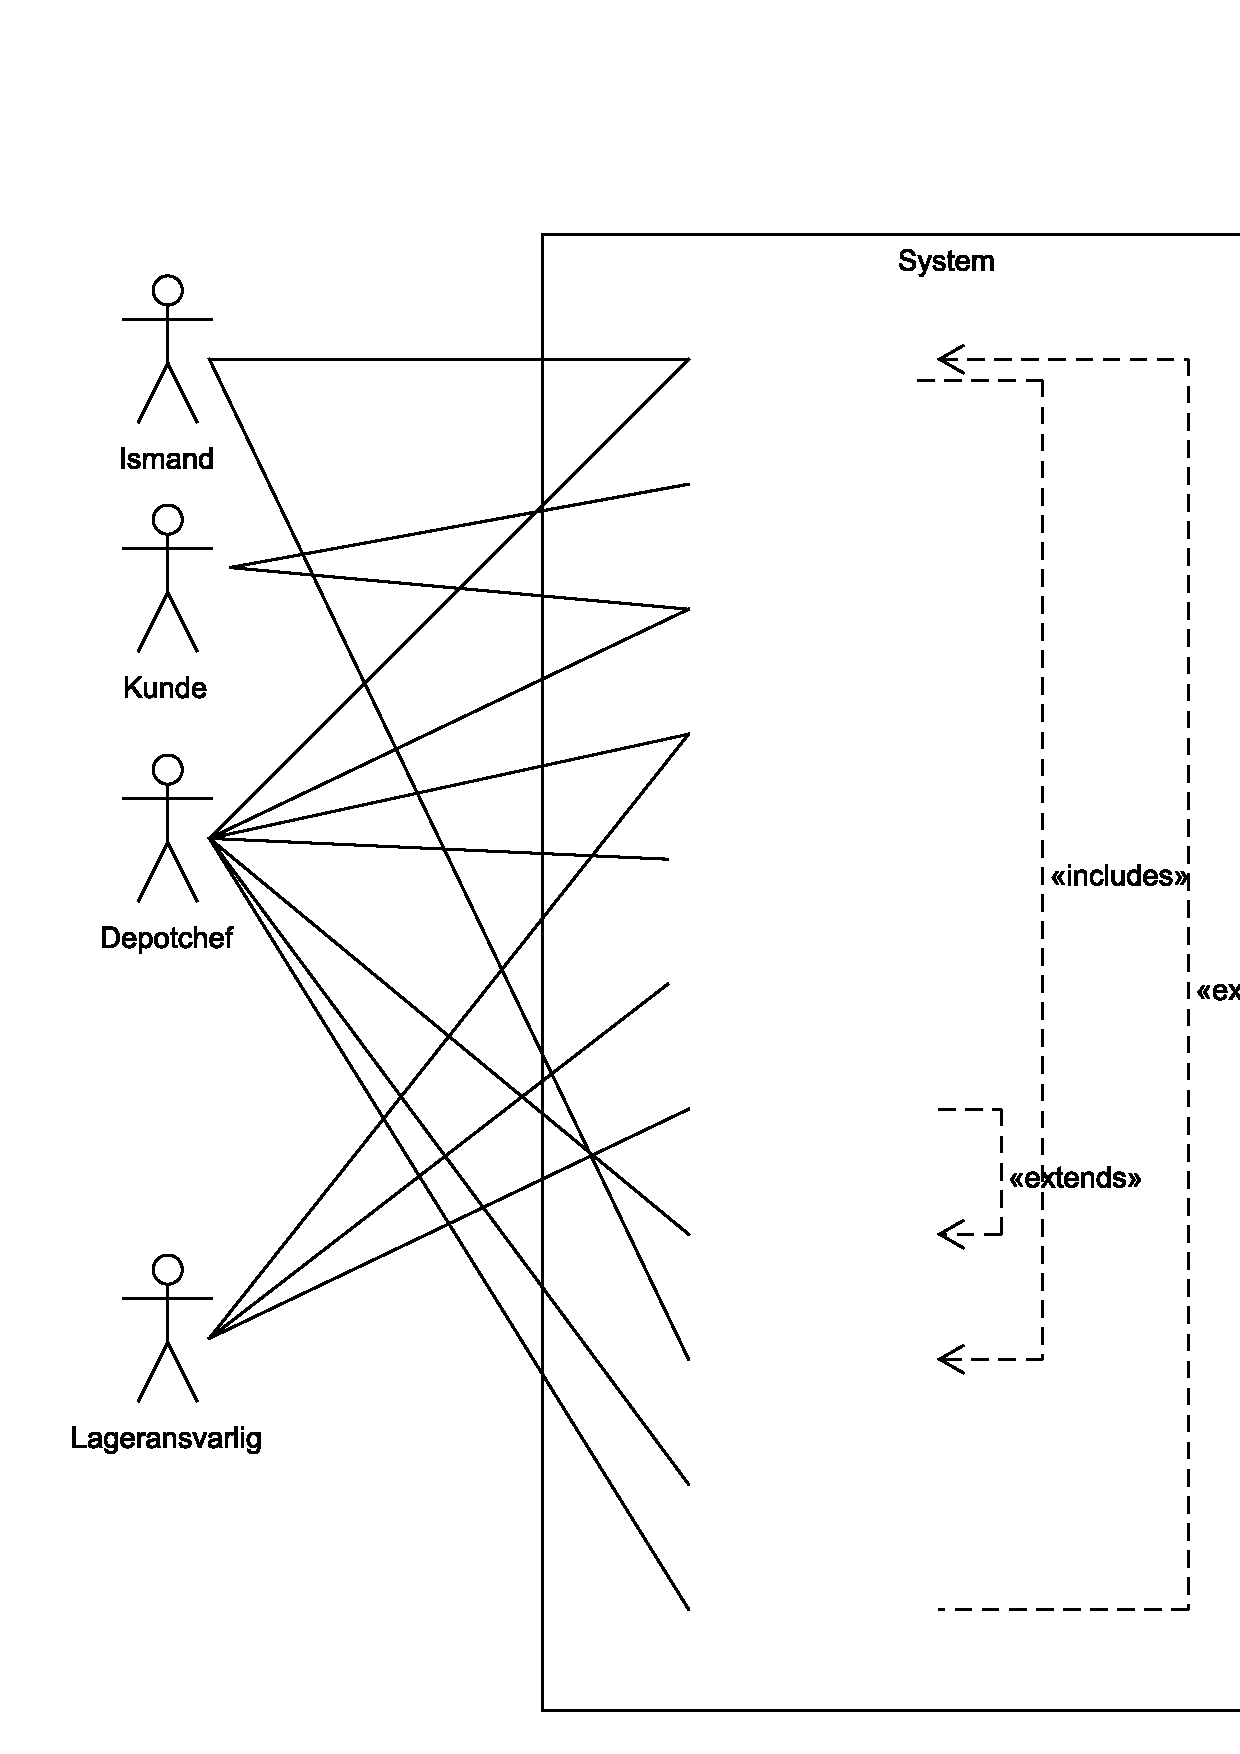
\includegraphics[width=\textwidth]{figures/Forundersøgelse/use_case_diagram.png}
    \caption{Use case diagram}
    \label{fig:use_case_diagram}
\end{figure}

\begin{figure}[H]
    \centering
    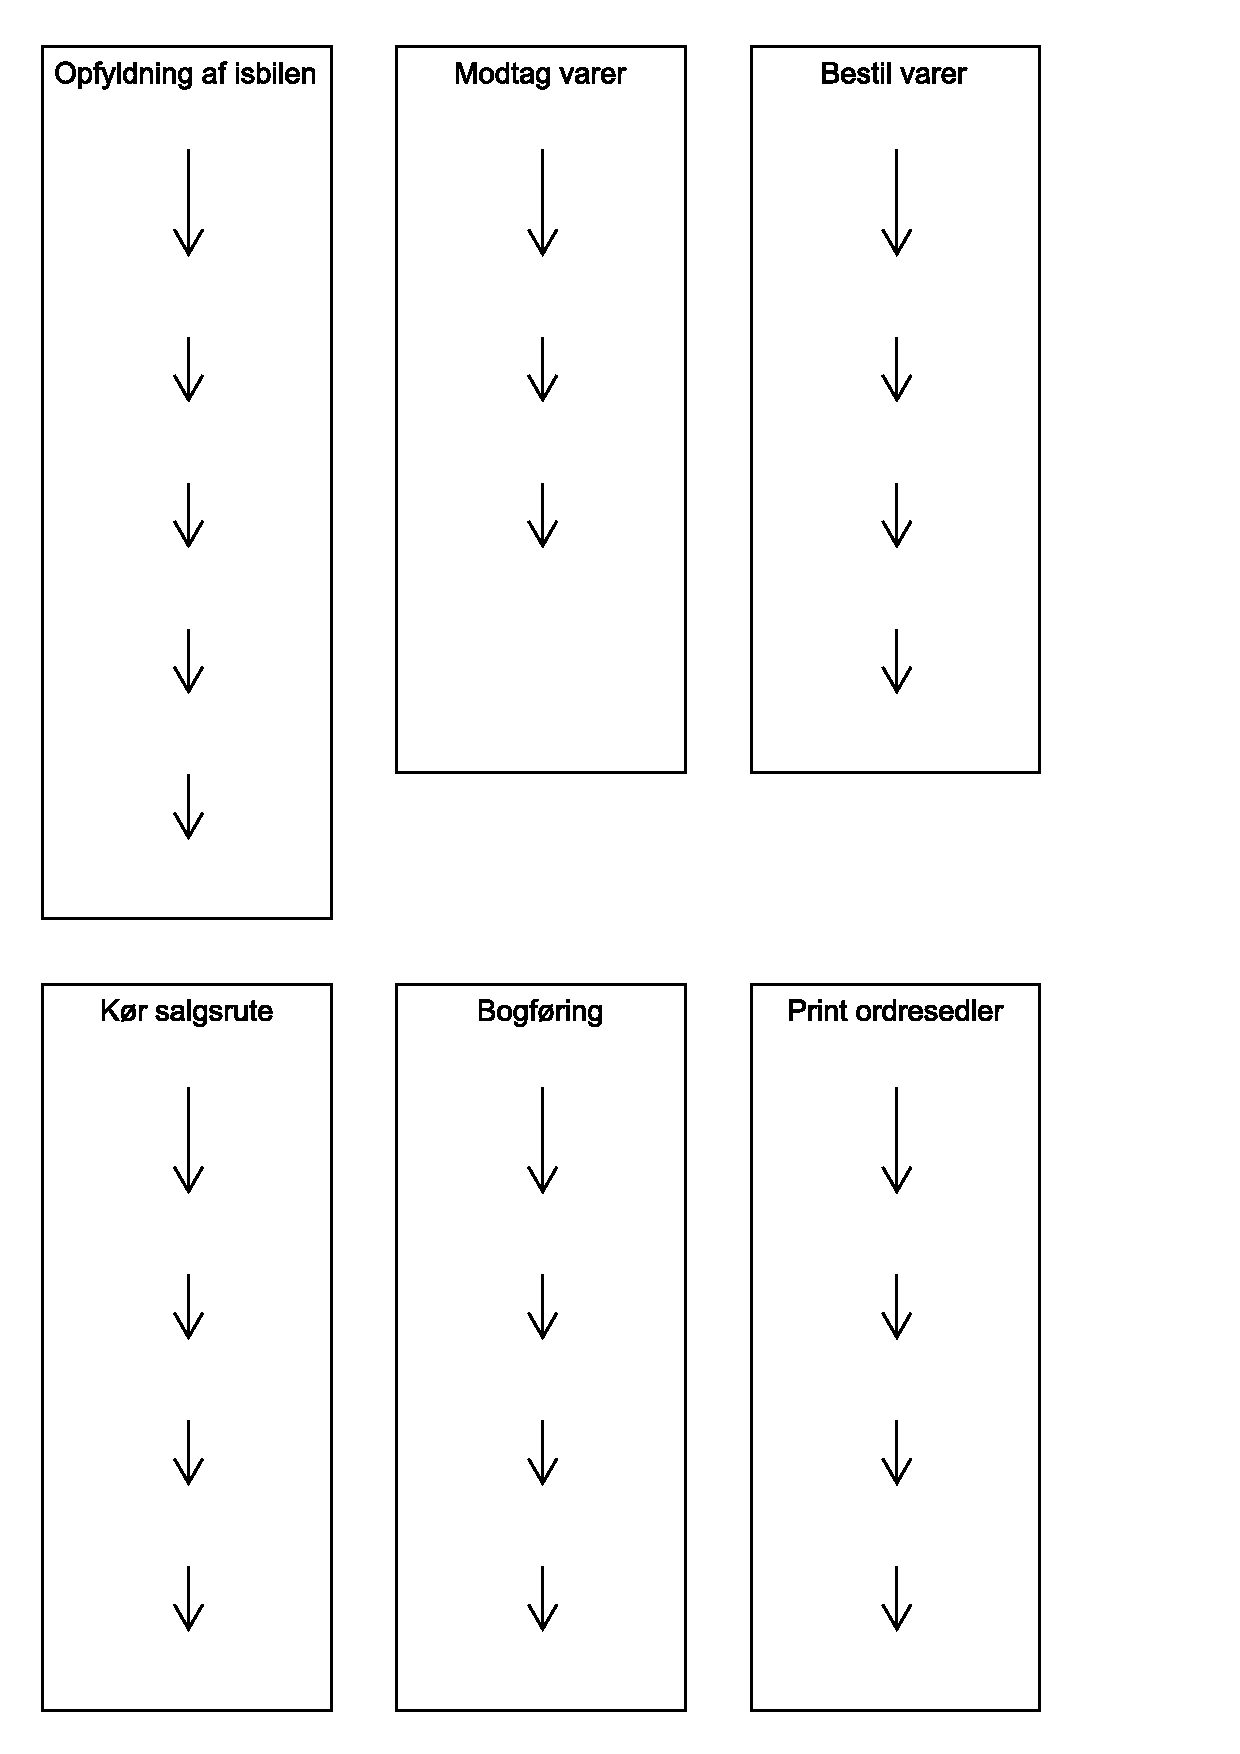
\includegraphics[width=\textwidth]{figures/Forundersøgelse/workflows.png}
    \caption{Workflow diagram}
    \label{fig:workflows}
\end{figure}